В данном блоке приведены примеры работы сети с протоколом повторной отправки GBN, вероятности потери 0.2, а также с окном, равному 5. Исходные данные делились на 63 фрагмента.

\subsection{Топология ``Линейная''}

Линейная топология представляет из себя 7 узлов, соединенных в одну линию шестью ребрами. Формально выглядит так:
\begin{itemize}
    \item Вершины: [0, 1, 2, 3, 4, 5, 6]
    \item Соседи: [[1], [0, 2], [1, 3], [2, 4], [3, 5], [4, 6], [5]]
\end{itemize}

После разбиения тестового файла на фрагменты и загрузки фрагментов на данные 7 узлов, можно увидеть такое распределение частей, как на \ref{fig:lin-files}. Как видно, сами фрагменты на каждом отдельном роутере дают мало понимания о том, что за файл хранится на роутерах. Рассмотрим результат работы при сборке фрагментов для крайнего (нулевого) и центрального (третьего) узлов. 

\begin{figure}[H]
    \centering
    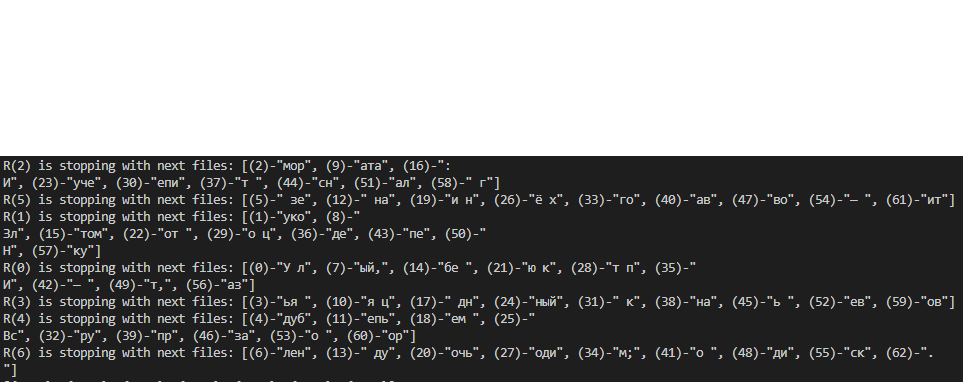
\includegraphics[width=0.88\linewidth]{imgs/lin-files.png}
    \caption{Разбиение файла на фрагменты и их распределения на роутерах}
    \label{fig:lin-files}
\end{figure}

Как видно из рисунков \ref{fig:lin-res-0} и \ref{fig:lin-res-1} - за этими фрагментами прятались вполне известные строчки вполне известного произведения. Однако видно еще и то, что время работы для центрального узла меньше почти в 2 раза: это можно попытаться обяснить тем, что суммарный путь пройденный пакетами во втором случае больше, чем для первого. А чем больше путь, тем больше пересылок по каналам связи с потерями было осуществлено. Однако, для более точных выводов, нужно производить большую серию замеров и усреднение. 

\begin{figure}[H]
    \centering
    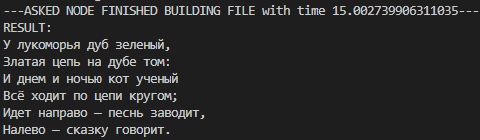
\includegraphics[width=0.88\linewidth]{imgs/lin-res-0.png}
    \caption{Результат сборки файла для нулевого (крайнего) узла прямой}
    \label{fig:lin-res-0}
\end{figure}

\begin{figure}[H]
    \centering
    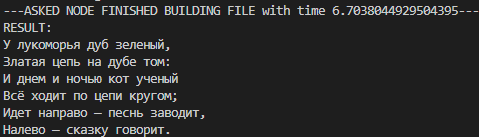
\includegraphics[width=0.88\linewidth]{imgs/lin-res-3.png}
    \caption{Результат сборки файла для третьего (центрального) узла прямой}
    \label{fig:lin-res-3}
\end{figure}

\subsection{Топология ``Звезда''}

В данном случае была рассмотрена следующая топология:
\begin{itemize}
    \item Вершины: [0, 1, 2, 3, 4]
    \item Соседи: [[1, 2, 3, 4], [0], [0], [0], [0]]
\end{itemize}
Как видно, нулевой узел здесь является центральным, а все остальные - ``лучами'' получаемой сети.

Рассмотрим содержимое роутеров после разбиения того же файла на фрагменты и их распределения по узлам. На рис. \ref{fig:star-files} видны те же фрагменты, однако для каждый роутер хранит большее число фрагментов, чем в предыдущем случае. Рассмотрим результаты.

\begin{figure}[H]
    \centering
    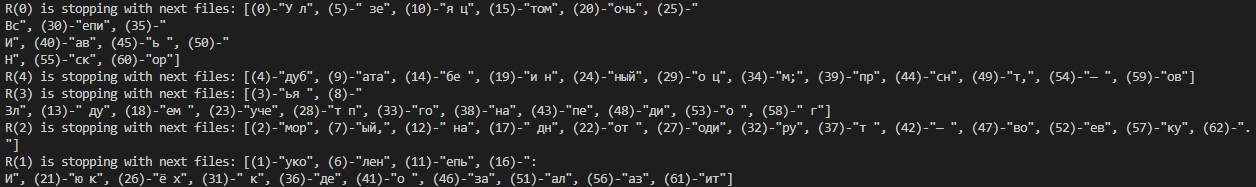
\includegraphics[width=0.88\linewidth]{imgs/star-files.png}
    \caption{Разбиение файла на фрагменты и их распределения на роутерах для звезды}
    \label{fig:star-files}
\end{figure}

Рисунки \ref{star-res-1} и \ref{star-res-0} отображают тот же результат, только другие времена, в сравнении с предыдущим опытом.

\begin{figure}[H]
    \centering
    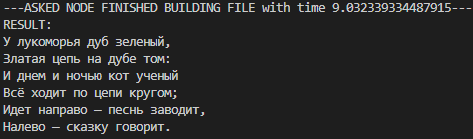
\includegraphics[width=0.88\linewidth]{imgs/star-res-0.png}
    \caption{Результат сборки файла для нулевого (центрального) узла звезды}
    \label{star-res-0}
\end{figure}

\begin{figure}[H]
    \centering
    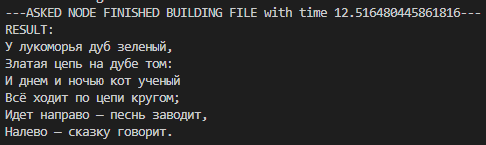
\includegraphics[width=0.88\linewidth]{imgs/star-res-1.png}
    \caption{Результат сборки файла для первого (лучевого) узла звезды}
    \label{star-res-1}
\end{figure}

\subsection{Топология ``Кольцо''}

В данном случае была рассмотрена следующая топология:
\begin{itemize}
    \item Вершины: [0, 1, 2, 3, 4, 5, 6]
    \item Соседи: [[6, 1], [0, 2], [1, 3], [2, 4], [3, 5], [4, 6], [5, 0]]
\end{itemize}
Все узлы имеют два соседа с индексами, отличающихся на 1 - данная топология является кольцом. В данном случае достаточно рассмотреть 1 случай работы для произвольного узла.

Содержимое роутеров после разбиения файла на фрагменты и распределения по узлам представлена на рис. \ref{fig:star-files}. Рассмотрим результаты сборки.

\begin{figure}[H]
    \centering
    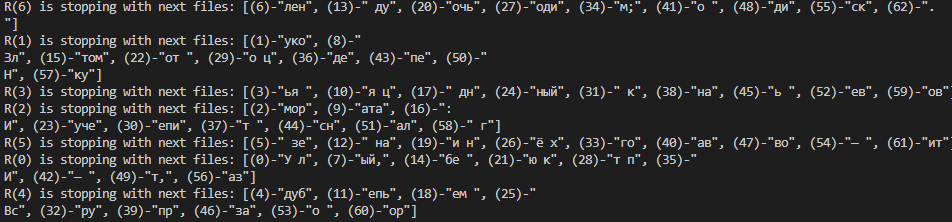
\includegraphics[width=0.88\linewidth]{imgs/circle-files.png}
    \caption{Разбиение файла на фрагменты и их распределения на роутерах для кольца}
    \label{fig:circle-files}
\end{figure}

Рисунок \ref{circle-res} отображает корректность работы симуляции.

\begin{figure}[H]
    \centering
    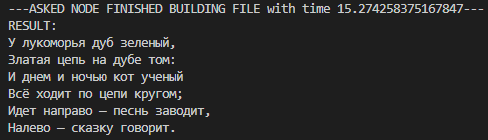
\includegraphics[width=0.88\linewidth]{imgs/circle-res.png}
    \caption{Результат сборки файла для нулевого (произвольного) узла кольца}
    \label{circle-res}
\end{figure}
